
\begin{frame}
    \frametitle{In a nutshell}

    \LARGE
    \centering

    We want \alert{fully compositional} and \alert{mathematically rigorous}
    foundation for reasoning about circuits

    \vspace{1em}

    \dsptikzfig{strings/category/composition}[colour=seq]
    \dsptikzfig{strings/monoidal/tensor}[colour=seq]
    \dsptikzfig{strings/traced/trace-rhs}[colour=seq]

\end{frame}

\section{Part I: Semantics of Digital Circuits}

\begin{frame}

    \Huge
    \centering

    \pause
    Part I

    \pause

    \textbf{Semantics of Digital Circuits}

    \Large
    \vspace{0.25em}

    \pause

    Refining the previous work on categorical digital circuits, leading to
    three \alert{sound and complete} notions of semantics

    \large
    \vspace{0.5em}

    \pause

    Ghica, K., and Sprunger, 2024. \\
    \textbf{A Fully Compositional Theory of Sequential Digital Circuits}

\end{frame}

\begin{frame}
    \frametitle{Previously, on circuits}

    \pause

    \begin{minipage}{0.65\textwidth}
        First steps...

        \vspace{0.5em}

        Lafont, 2003. \\
        \textbf{Towards an algebraic theory of Boolean circuits}
    \end{minipage}
    \quad
    \begin{minipage}{0.3\textwidth}
        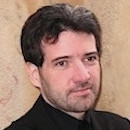
\includegraphics[width=0.33\textwidth]{lafont}
    \end{minipage}

    \vspace{2em}

    \pause

    \begin{minipage}{0.65\textwidth}
        More recently...

        \vspace{0.5em}

        Ghica and Jung, 2016. \\
        \textbf{Categorical Semantics of Digital Circuits}

        Ghica, Jung, and Lopez, 2017. \\
        \textbf{Diagrammatic Semantics for Digital Circuits}
    \end{minipage}
    \quad
    \begin{minipage}{0.3\textwidth}
        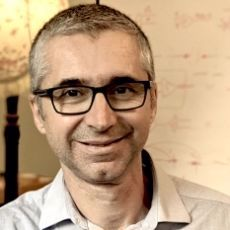
\includegraphics[width=0.32\textwidth]{ghica}
        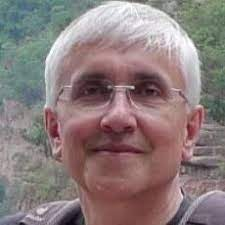
\includegraphics[width=0.32\textwidth]{achim}
        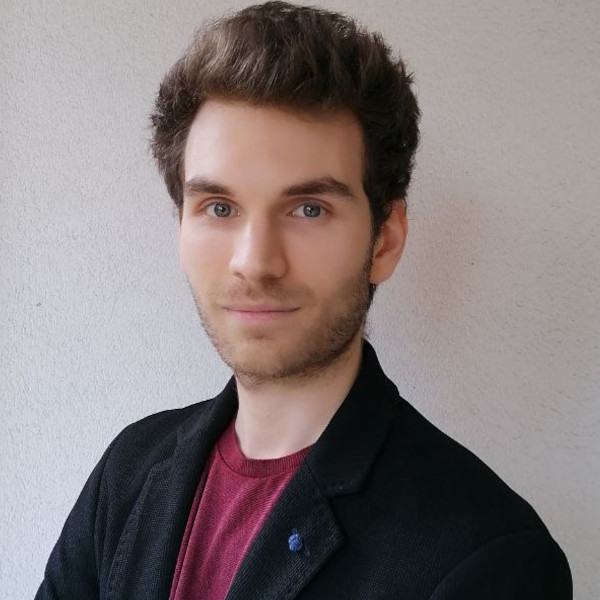
\includegraphics[width=0.32\textwidth]{lopez}
    \end{minipage}

\end{frame}

\begin{frame}
    \frametitle{Chapter 3: Syntax}

    \pause

    \textbf{Previously:} syntax and semantics confusingly intermingled with
    layers of quotients and equations

    \pause

    \textbf{Now:} syntax of circuits defined before considering any behaviour

    \pause

    \vspace{1em}

    \begin{center}
        \begin{minipage}{0.4\textwidth}
            \centering
            {\LARGE\(\ccircsigma\)}

            \vspace{1em}

            \alert{Combinational} circuits

            (functions)
        \end{minipage}
        \pause
        {\LARGE\(\hookrightarrow\)}
        \begin{minipage}{0.4\textwidth}
            \centering
            {\LARGE\(\scircsigma\)}

            \vspace{1em}

            \alert{Sequential} circuits

            (stateful)
        \end{minipage}
    \end{center}

\end{frame}

\begin{frame}
    \frametitle{Chapter 4: Denotational semantics}

    \pause

    \textbf{Previously:} denotations of circuits only considered informally

    \pause

    \textbf{Now:} assign behaviour to circuit morphisms in terms of
    \alert{causal, monotone, and finitely specified stream functions} using
    a construction via \alert{Mealy machines}

    \pause

    \vspace{1em}

    \begin{center}
        \begin{minipage}{0.15\textwidth}
            \centering
            {\LARGE\(\scircsigma\)}
        \end{minipage}
        \pause
        \(\xrightarrow{\circuittomealyi}\)
        \begin{minipage}{0.25\textwidth}
            \centering
            {\LARGE\(\mealyi\)}

            \vspace{0.5em}

            \alert{Monotone} Mealy machines
        \end{minipage}
        \pause
        \(\xrightarrow{\mealytocircuiti}\)
        \begin{minipage}{0.375\textwidth}
            \centering
            {\LARGE\(\streami\)}

            \vspace{0.5em}

            \alert{Causal, monotone, finitely specified} stream functions
        \end{minipage}
    \end{center}

\end{frame}

\begin{frame}
    \frametitle{Chapter 4: Denotational semantics}

    \pause

    \begin{center}
        \LARGE
        \(\scircsigma \xrightarrow{\circuittostreami} \streami\)
    \end{center}

    \pause

    \[
        \circuittostreami[
            \dsptikzfig{strings/category/f}[box=f,colour=seq]
        ]
        =
        \circuittostreami[
            \dsptikzfig{strings/category/f}[box=g,colour=seq]
        ]
        \quad
        \Rightarrow
        \quad
        \dsptikzfig{strings/category/f}[box=f,colour=seq]
        \extequivi
        \dsptikzfig{strings/category/f}[box=g,colour=seq]
    \]

    \pause

    \begin{center}
        \LARGE
        \alert{Denotational equivalence}

        \vspace{1em}

        \(\scircsigmai \cong \streami\)
    \end{center}


\end{frame}

\begin{frame}
    \frametitle{Chapter 5: Operational semantics}

    \pause

    \textbf{Previously:} reduction strategy for \alert{closed} circuits with
    \alert{delay-guarded} feedback

    \pause

    \textbf{Now:} reduction strategy for any \alert{open} circuit using novel
    rule for \alert{unrolling non-delay-guarded feedback}

    \pause

    \[
        \dsptikzfig{circuits/instant-feedback/equation-lhs}[box=f]
        \reduction
        \dsptikzfig{circuits/instant-feedback/concrete-unfolding}[box=f]
    \]

    \vspace{0.5em}

    \pause

    \scalebox{0.9}{
        \(
        \dsptikzfig{circuits/productivity/productive-goal-lhs}[box=f]
        \reduction
        \dsptikzfig{circuits/productivity/mealy-form-applied}[core=\hat{f}]
        \reduction
        \dsptikzfig{circuits/productivity/mealy-form-instant-registers}[core=\hat{f}]
        \reduction
        \dsptikzfig{circuits/productivity/productive-goal-rhs}[box=g]
        \)
    }

\end{frame}

\begin{frame}
    \frametitle{Chapter 5: Operational semantics}

    \pause

    \begin{center}
        \begin{minipage}{0.55\textwidth}
            \centering
            \dsptikzfig{strings/category/f}[box=f,colour=seq]
            and
            \dsptikzfig{strings/category/f}[box=g,colour=seq]
            produce the same

            \vspace{0.5em}

            outputs using the productive
            strategy
        \end{minipage}
        \quad
        \(\Rightarrow\)
        \begin{minipage}{0.3\textwidth}
            \centering
            \(
            \dsptikzfig{strings/category/f}[box=f,colour=seq]
            \sim_{\interpretation}
            \dsptikzfig{strings/category/f}[box=g,colour=seq]
            \)
        \end{minipage}
    \end{center}

    \vspace{0.25em}

    \pause

    \begin{center}
        \LARGE
        \alert{Observational equivalence}

        \vspace{0.5em}

        \(
        \dsptikzfig{strings/category/f}[box=f,colour=seq]
        \sim_{\interpretation}
        \dsptikzfig{strings/category/f}[box=g,colour=seq]
        \Leftrightarrow
        \dsptikzfig{strings/category/f}[box=f,colour=seq]
        \extequivi
        \dsptikzfig{strings/category/f}[box=g,colour=seq]
        \)

        \vspace{0.5em}

        \(\scircsigmaobs \cong \scircsigmai\)
    \end{center}
\end{frame}

\begin{frame}
    \frametitle{Chapter 6: Algebraic semantics}

    \pause

    \textbf{Previously:} circuits quotiented by certain `natural laws', along
    with quotients of `extensional equivalence' to add in remaining equalities

    \pause

    \textbf{Now:} set of equations \(\mce_\interpretation\) guided by the stream
    semantics; some local interactions and some `contextual' equations

    \pause

    \begin{center}
        \LARGE
        \(
        \dsptikzfig{strings/category/f}[box=f,colour=seq]
        =_{\mce_\interpretation}
        \dsptikzfig{strings/category/f}[box=g,colour=seq]
        \Leftrightarrow
        \dsptikzfig{strings/category/f}[box=f,colour=seq]
        \extequivi
        \dsptikzfig{strings/category/f}[box=g,colour=seq]
        \)

        \vspace{0.5em}
        \pause
        \(\scircsigmae \cong \scircsigmai\)
    \end{center}


\end{frame}

\begin{frame}
    \frametitle{Chapter 7: Potential applications}

    \pause

    Primarily \alert{theoretical}, but have also considered potential
    \alert{applications}

    \pause

    Ideas to \alert{complement} existing circuit technologies rather than
    \alert{replace} them

    \large
    \vspace{0.5em}

    \pause

    \begin{center}
        \begin{minipage}{0.45\textwidth}
            \textbf{Partial evaluation}
            \centering

            \vspace{0.25em}

            Fixing some inputs and reducing circuits accordingly

        \end{minipage}
        \quad\pause
        \begin{minipage}{0.45\textwidth}
            \centering
            \textbf{Refining circuits}

            \vspace{0.25em}

            Using (in)equational reasoning to improve circuit performance
        \end{minipage}

        \pause
        \vspace{1em}

        \begin{minipage}{0.45\textwidth}
            \centering
            \textbf{Layers of abstraction}

            \vspace{0.25em}

            Working at different abstractions in the same diagram
        \end{minipage}
        \quad\pause
        \begin{minipage}{0.45\textwidth}
            \centering
            \textbf{Tidying}

            \vspace{0.25em}

            Automatically remove redundant parts of circuits

        \end{minipage}
    \end{center}

\end{frame}

\begin{frame}
    \frametitle{Intermission}

    \centering
    \Large

    \pause

    This fulfils our \alert{original goal} of a mathematically rigorous
    theory of digital circuits

    \pause
    \vspace{1em}

    But this is not very useful for \alert{real world} circuits, which are
    very complicated

    \pause
    \vspace{1em}

    We want to be able to \alert{automate} reasoning with digital circuits

\end{frame}

\section{Part II: Graph Rewriting for Digital Circuits}

\begin{frame}

    \Huge
    \centering

    Part II

    \textbf{Graph Rewriting for Digital Circuits}

    \Large
    \vspace{0.25em}

    Adapting recent work on \alert{hypergraph string diagram rewriting} for
    settings with a \alert{traced comonoid} structure

    \large
    \vspace{0.5em}

    \pause

    Ghica and K., 2023. \\
    \textbf{Rewriting Modulo Traced Comonoid Structure}

\end{frame}

\begin{frame}
    \frametitle{Previously, on graphs}

    \pause

    \begin{minipage}{0.65\textwidth}
        Bonchi et al, 2016. \\ \textbf{Rewriting Modulo Symmetric Monoidal Structure}
    \end{minipage}
    \quad
    \begin{minipage}{0.3\textwidth}
        
\includegraphics[width=0.32\textwidth]{bonchi}
        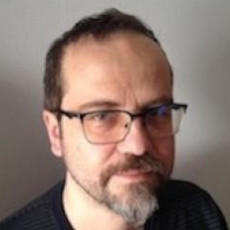
\includegraphics[width=0.32\textwidth]{gadduchi}
        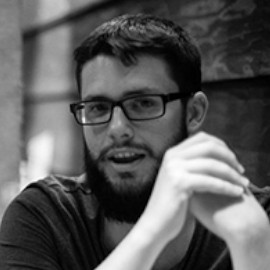
\includegraphics[width=0.32\textwidth]{kissinger}
        
\includegraphics[width=0.32\textwidth]{sobocinski}
        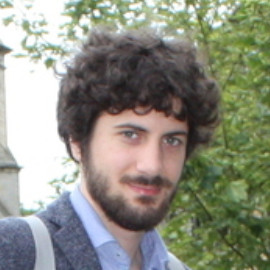
\includegraphics[width=0.32\textwidth]{zanasi}
    \end{minipage}

    \vspace{2em}
    \pause

    \begin{minipage}{0.65\textwidth}
        Ghica, Jung and Lopez, 2017. \\ \textbf{Diagrammatic Semantics for Digital Circuits}
    \end{minipage}
    \quad
    \begin{minipage}{0.3\textwidth}
        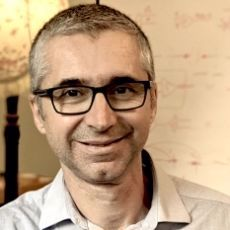
\includegraphics[width=0.32\textwidth]{ghica}
        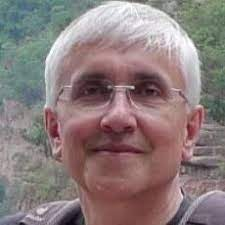
\includegraphics[width=0.32\textwidth]{achim}
        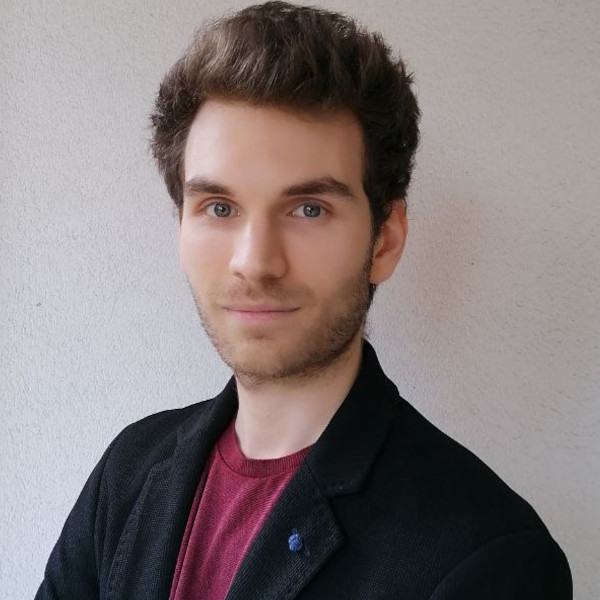
\includegraphics[width=0.32\textwidth]{lopez}
    \end{minipage}

\end{frame}

\begin{frame}
    \frametitle{Chapter 8: String diagrams as hypergraphs}

    \pause

    \textbf{Bonchi et al:}
    String diagrams encoded as \alert{cospans of hypergraphs}

    \pause

    Arbitrary cospans correspond to terms with a \alert{Frobenius} structure

    \pause

    \alert{Monogamous acyclic} cospans correspond to
    \alert{symmetric monoidal} terms

    \vspace{2em}

    \pause

    \textbf{This work:}
    Define notion of \alert{partial monogamy} and \alert{partial left-monogamy}

    \pause

    \alert{Partial monogamous} cospans correspond to
    \alert{traced} terms

    \pause

    \alert{Partial left-monogamous} cospans correspond to
    \alert{traced comonoid} terms
\end{frame}

\begin{frame}
    \frametitle{String diagrams as hypergraphs}

    \pause

    \begin{center}
        \begin{minipage}{0.4\textwidth}
            \centering
            \LARGE
            \(\pmcspdhyp\)

            \Large
            Partial monogamous cospans of hypergraphs

            \vspace{0.5em}

            \dsptikzfig{graphs/partial-monogamy/yes-0}
        \end{minipage}
        \qquad
        \pause
        {\LARGE \(\cong\)}
        \begin{minipage}{0.4\textwidth}
            \centering
            \LARGE
            \(\stmcsigma\)

            \Large
            Traced terms

            \vspace{1em}

            \dsptikzfig{graphs/terms/term-0}
        \end{minipage}
    \end{center}
\end{frame}

\begin{frame}
    \frametitle{Chapter 8: String diagrams as hypergraphs}

    \pause

    \begin{center}
        \begin{minipage}{0.4\textwidth}
            \centering
            \LARGE
            \(\pmcspdhyp\)

            \Large
            Partial monogamous cospans of hypergraphs

            \vspace{0.5em}

            \dsptikzfig{graphs/partial-monogamy/yes-comonoid-0}
        \end{minipage}
        \qquad
        \pause
        {\LARGE \(\cong\)}
        \qquad
        \begin{minipage}{0.4\textwidth}
            \centering
            \LARGE
            \(\stmcsigma + \ccomon\)

            \Large
            Traced comonoid terms

            \vspace{1em}

            \normalsize
            \dsptikzfig{graphs/terms/comonoid-term-0}
        \end{minipage}
    \end{center}
\end{frame}

\begin{frame}
    \frametitle{Chapter 9: Graph rewriting}

    \pause

    Valid graph rewrites for an occurrence of a rule in a graph determined by
    presence of \alert{pushout complements}

    \vspace{1em}

    \pause

    \textbf{Bonchi et al:}
    \alert{Every} pushout complement corresponds to a Frobenius rewrite

    \alert{Exactly one} pushout complement corresponds to a symmetric
    monoidal rewrite

    \vspace{1em}

    \pause

    \textbf{This work:}

    \alert{Partial boundary complements} correspond to \alert{traced}
    rewrites

    \alert{Partial left-boundary complements} correspond to
    \alert{traced comonoid} rewrites

\end{frame}

\begin{frame}
    \frametitle{Chapter 10: Applications of graph rewriting}

    \pause

    Have developed \alert{hardware description language} for
    \alert{automatically} evaluating circuits using graph rewriting

    \pause

    \vspace{0.5em}

    \begin{center}
        \includesvg[width=0.85\textwidth]{figures/circuits/hdl/latch}

        \vspace{0.5em}

        \includesvg[width=0.85\textwidth]{figures/circuits/hdl/latch-outputs}
    \end{center}
\end{frame}

\begin{frame}
    \frametitle{Conclusion}

    \pause

    \Large
    \centering

    Two broad themes...

    \pause

    \vspace{1em}

    A \alert{fully compositional} theory of digital circuits, comprising
    \alert{denotational}, \alert{operational}, and \alert{algebraic} semantics

    \pause

    \vspace{1em}

    The setting in which we can perform \alert{graph rewriting} with digital
    circuits to automate reasoning

\end{frame}

\begin{frame}
    \frametitle{Future work}
    \centering

    \pause

    Some possible future avenues...

    \Large
    \pause
    \textbf{Theoretical extensions}

    \large

    Formalise \alert{partial evaluation} techniques or \\
    \alert{inequational} reasoning with circuits

    \Large
    \pause
    \textbf{More applications}

    \large
    Bring the theoretical blueprints to \alert{verifying} and \\
    \alert{synthesising} industry-grade circuits

    \Large
    \pause
    \textbf{Beyond the abstraction}

    \large
    Move to continuous signals or time \\
    (propagation delay, amplifiers, asynchronicity?)

\end{frame}